\documentclass[answers, 12pt]{article}

% import a set of useful packages for math
\usepackage{amsmath, amsfonts, amssymb}

% this package makes margins smaller
\usepackage{fullpage}

% for importing images
\usepackage{graphicx}

%%%% import any other packages here
\usepackage[parfill]{parskip} 

\usepackage{algorithmic}
\usepackage{algorithm}
\usepackage{float}
\usepackage{physics}
\usepackage[final]{pdfpages}
\usepackage{qcircuit}

%%%% make any other definitions here
\newcommand{\set}[1]{\left\{ #1 \right\}}
\newcommand{\Set}[1]{\big\{ #1 \big\}}


%%%%%%%%%%%%%%%%%%%%%%%%%%%%%%%%
\begin{document}

\title{CSCI 7000: Advanced Data Structures (Assignment 1)}
\author{Nicholas Papadopoulos}
\date{\today}
\maketitle


%%%%%%%%%%%%%%%%
\section*{Problem 1}
\subsection*{Part A}

\begin{align*}
  x_1 \oplus x_2 &= x_1 \oplus x_3 \\
  x_1 \oplus x_1 \oplus x_2 &= x_1 \oplus x_1 \oplus x_3 \\
  x_2 &= x_3 \\
\end{align*}

So, we need to find the probability that $x_2 = x_3$. There are $2^l$ possibile bitsrings of length $l$, so the probability that the same bitstring is randomly generated for both $x_2$ and $x_3$ is $\boldsymbol{\frac{1}{2^l}}$.


\subsection*{Part B}

Set $x_1 \oplus x_2$ can map to some other random string, say $s$. Each bitstring, $s$, of length $l$ can have $2^l$ pairs, where order matters, that xor to $s$. This is because you can choose any random bitstring, $r$, of length $l$, xor it with $s$, and the result, $r^\prime$ will be the paired value of $r$ where $r oplus r^\prime = s$. In other words, any random string out of the possible $2^l$ strings can serve as $x_3$ with a deterministic, corresponding $x_4$.

Hence, $x_1$, $x_2$, and $x_3$ can be anything without consequence. With these set, however, we know that $x_4 = x_1 \oplus x_2 \oplus x_3$. In other words, there is only one possible solution for $x_4$ once the free variables $x_1$, $x_2$, and $x_3$ are chosen. Since $x_4$ is chosen randomly, and there are $2^l$ possible choices, the probability that $x_1 \oplus x_2 = x_3 \oplus x_4$ is $\boldsymbol{\frac{1}{2^l}}$.


\subsection*{Part C}

First, we can determine the probability that $x$ maps to the same keys for $A$ and $B$. That is, what is the probability that $x_1 = x_2$? We have determined that this probability is $\frac{1}{2^l}$ in part (A).

\begin{align*}
  h_{A,B}(x) &= A[x_1] \oplus B[x_1] \\
  h_{A,B}(y) &= A[y_1] \oplus B[y_1] \\
\end{align*}

We can now ask what the probability is that $A[x_1] \oplus B[x_1] =A[y_1] \oplus B[y_1]$. Since $A[x_1]$, $A[x_2]$, $A[y_1]$, and $A[y_1]$ are random $l$-bit strings, we can use our answer in part (B) to say that the probability of collision is $\frac{1}{2^l}$.


%%%%%%%%%%%%%%%%
\section*{Problem 2}

\begin{align*}
  h_1(x) &= (x \mod 6) \mod 4 \\
  h_2(x) &= (2x \mod 6) \mod 4 \\
  h_3(x) &= (3x \mod 6) \mod 4 \\
  h_4(x) &= (4x \mod 6) \mod 4 \\
  h_5(x) &= (5x \mod 6) \mod 4 \\
\end{align*}

Here, we can see that we can pick $h_3$ and see that 

\[
  h_3(x) = \begin{cases}
    0 & x \text{ is even} \\
    3 & x \text{ is odd}
  \end{cases}
\]

This is because 3 times any even number will be exactly divisible by 6, giving a remainder of 0, and 3 times and odd number will be 3 times and even number plus 3, giving a remainder of 3. Since both 0 and 3 are less than 4, modding by 4 does not effect the result. Hence, $\frac{1}{2}$ off the possible keys to $h_3$ will result in the same answer, so there the probability of a collision is $\boldsymbol{\frac{1}{2} > \frac{1}{4}}$.


%%%%%%%%%%%%%%%%
\section*{Problem 3}

We can take the binary representation of each character and mod them by some number, say 10. Then we can multiply each character by subsequent powers of ten so that no character can interfere with the next when added together, since the highest value of some power, $p$, $9 * 10^p < 10^{p+1}$. This holds true for any base, say $a$, not only 10. In order to ensure some value for each character, we can mod by $a - 1$ and add 1 to the result. We can use this fact to include a salt, so we can say that 

\[
  a = b + \texttt{salt}
\]

Where $b$ is some minimum base number we would like to utilize. We can then define a character encoding by

\[
  (x_n = c_n \mod (a - 1)) + 1
\]

We then have that 

\[
  h(s) = x_1(a^n) + x_2(a^{n-1}) + ... x_n(a^0)
\] 

 $h(t)$ would then be 
 
 \[
  h(t) = x_2(a^{n}) + x_3(a^{n-1}) + ... x_{n+1}(a^0)
\]

So, to retrieve $h(t)$ given $s$, $t$, and $h(s)$, we simply subtract $x_1(a^n)$, multiply the result by a, then add $x_{n+1}$.

 \[
  h(t) = (h(s) - x_1(a^n))a + x_{n+1}
\]

This uses constant time operations for all portions of this equation, consisting of modulo, exponentiation, subtraction, multiplication, and addition.


%%%%%%%%%%%%%%%%
\section*{Problem 4}
\subsection*{Explanation}
My solution first implements the naive version, where all substrings are stored in a hash table, with the key being the substring itself and the value being a list of indices where that substring was found. It begins at the first index of the first word, extracts the substring from that index of the given length, then inserts the substring into the hash along with the start index. It will then move to the next index and repeat until all substrings of the word have been stored in the set. It then repeats this process with the second word in a second hash table. Finally, it goes through each entry in one of the hash tables and determines if there is a matching substring in the second hash table by querying the key. If there is a matching key, it creates a set product of the two words' index lists, creating all possible combinations of start indices for both words that generate the same substring.

The more complex solution actually uses nearly the same algorithm, except it hashes the keys using the process described in problem 3 of this homework instead of using the substring directly. So, instead of extracting each substring at each start index for a word, it first hashes only the first substring. Then, it hashes subsequent keys by giving only the next character and the first character of the hash before it.

In order to ensure it was working properly, I created tests on key and corner case inputs (strings and substring length) with known outputs and ensured that both methods produced correct results. I then ran tests using large, randomly generated strings and ensured that both methods returned the same result.

\subsection*{Benchmarking}
To benchmark these methods, I compared each method with strings varying from length 1 to 1000. Each comparison was run using five different random substring lengths. I then plotted the average duration of the substring finding algorithm across those five random substrings lengths against the length of the full input strings.

\[
  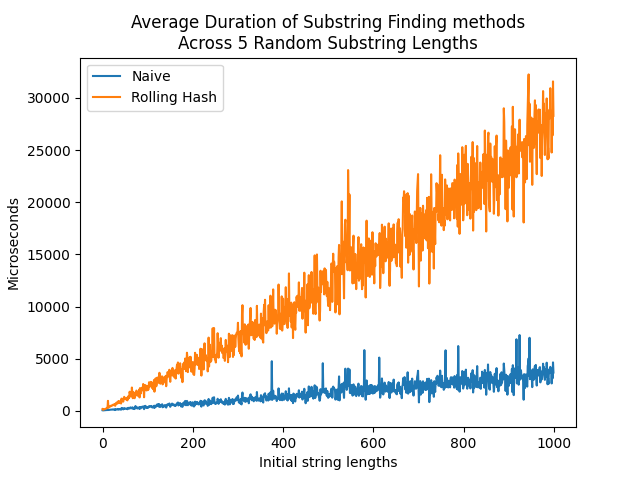
\includegraphics[width=0.5\textwidth]{images/durations.png}
\]

We can see here that the naive solution outperforms the complex version. We can speculate as to why this may be the case. First of all, there is an overflow error in the rolling hash, as the resulting integer is apparently too large. To resolve this, I experimented with different salts and modulo different locations. For example, instead of only modulo-ing the decimal value of a characer, I put a different, large, prime modulo on the result of all math operations. This solved the warning, but did not improve the duration with respect to the naive implementation.

I thought it may be due to some large number of unexpected collisions in the rolling hash function. As I debugged, though, I saw that the has sizes for both were identical during spot checks. However, I tried increasing the salt size, which would increase the modulo and allow for fewer collisions, just in case. This did not have any desirable effect. Here is the plot with a salt of 1000 instead of 100.

\[
  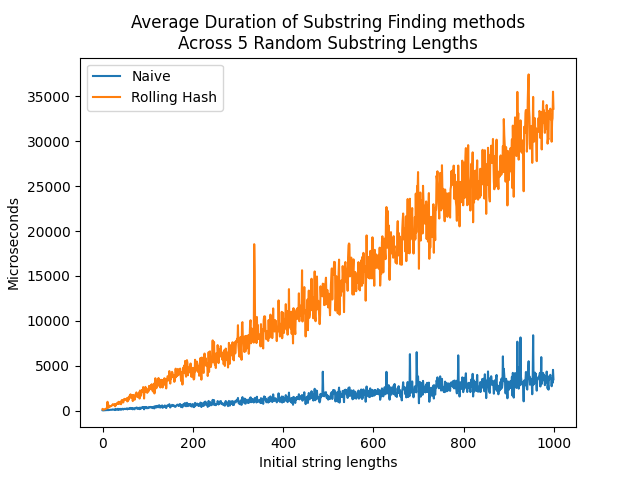
\includegraphics[width=0.5\textwidth]{images/durations_1000_salt.png}
\]

I speculate that the rolling hash function itself may take more operations to run than the naive counterpart. Perhaps there is a way to utilize the rolling hash function without storing all substring hashes of both strings when using the rolling hash. This would allow for fewer iteratons through the characters of the strings when using a rolling hash. Normally, we would expect the complexity of the naive function to be $O(n k)$, where $n$ is the length of the input strings and $k$ is the length of the substring. This is because for every character in $n$, we find a substring of length $k$ and insert it into the hash. For the rolling hash function, we would expect $O(n)$, because for ever character $n$, we perform a constant number of arithmetic operations. Since $n$ is the main culprit in the rolling hash function, it could potentially be further reduced by reducing the number of iterations through characters it must perform.

\end{document}
